\documentclass[portrait]{a0poster}
%\documentclass[landscape,final]{a0poster}
\usepackage{multicol}
\usepackage{amsfonts}
\usepackage{amsmath}
\usepackage{graphicx, color,wrapfig,sidecap}

\usepackage{txfonts}
\usepackage{tikz}


\usepackage{geometry}
\geometry{paperwidth=36in,paperheight=48in,margin=2in}

\setlength{\oddsidemargin}{1in}
\setlength{\evensidemargin}{1in}
\setlength{\columnsep}{1in}
\setlength{\topmargin}{1in}

%\setlength{\textwidth}{48in}
%\setlength{\textheight}{30.06in}
%\setlength{\textheight}{48in}


%\usepackage{pdftricks}
%\usepackage{graphicx}

\definecolor{turquoise}{cmyk}{0.65,0,0.1,0.1}
\definecolor{mygreen}{rgb}{0.2, 0.6, 0.6}
\definecolor{mygray}{rgb}{0.6, 0.6, 0.6}

\def\tcb{\textcolor{blue}}
\def\tcr{\textcolor{red}}
\def\tcg{\textcolor{mygreen}}
\def\tcgray{\textcolor{mygray}}

\usepackage{url}
\newtheorem{theorem}{Theorem}[section]
\newtheorem{lemma}[theorem]{Lemma}
\newtheorem{algorithm}{Algorithm}[section]
\newtheorem{definition}{Definition}[section]
\newtheorem{proposition}{Proposition}[section]
\newtheorem{remark}{Remark}

\def\a{\mathbf{a}}
\def\b{\mathbf{b}}
\def\c{\mathbf{c}}
\def\y{\mathbf{y}}
\def\e{\mathbf{e}}
\def\S{\mathbf{S}}
%%%%% Blackboard Bold Letters %%%%%%%%%%%%%%%%%%%%%%%%%%%%%%%%
\def\pp{\mathbb{P}}
\def\ee{\mathbb{E}}
\def\rr{{\mathbb R}}
\def\zz{{\mathbb Z}}
\def\rrn{{\mathbf R}^n}
\def\zzn{{\mathbb Z}^n}

%%% special symbols %%%%%%%%%%%%%
\def\xwig{\widetilde{X}}
\def\bPi{{\bf\Pi}}
\newcommand{\smallchoose}[2]{\mbox{${#1\choose #2}$}}
\def\dis{\displaystyle}
\def\M{\cal{M}}
\def\cbs{C_b(S)}
\def\cbr{C_b(\rr)}
\def\bs{\bigskip}
\def\bn{\bigskip\noindent}
\def\Gap{{\mathbf{Gap}}}
\def\h{{\mathbf h}}
\def\min{\mbox{min}}
\def\hp{\hat{\pi}}
\def\ii{{(i)}}
\def\hg{\hat{g}}
\def\xx{\mathcal{X}}
\def\Unif{\emph{Unif}}

\usepackage[usenames,dvipsnames]{pstricks}
\usepackage{epsfig}
\usepackage{pst-grad} % For gradients
\usepackage{pst-plot} % For axes

\definecolor{gray}{RGB}{175,175,175}
\def\tcr{\textcolor{red}}
\def\tcb{\textcolor{blue}}
\def\kk{{(k)}}
%\def\dir{/Users/yguan/Dropbox/work/vaccine/latex/}
%\def\dirquan{/Users/yongtaog/Dropbox/Shared/quan/selection/pic}




% I want to define section headings to be blue and bold.
\makeatletter
\renewcommand\section{\@startsection {section}{1}{\z@}%
                                   {-3.5ex \@plus -1ex \@minus -.2ex}%
                                   {2.3ex \@plus.2ex}%
                                   {\Large\bfseries\sc\color{blue}}}
\renewcommand\subsection{\@startsection {subsection}{2}{\z@}%
                                   {-3.5ex \@plus -1ex \@minus -.2ex}%
                                   {1.5ex \@plus.2ex}%
                                   {\large\bfseries\sc\color{mygreen}}}
\makeatother





%\title{Making a poster in \LaTeX}

%A unified framework of association mapping for admixed samples
%Admixed samples provide great opportunities in disease association mapping. First, the variation of local ancestry across individuals provide "free" genetic variates to be associatd with disease phenotypes. Second, the local ancestry of each marker serves as a background for genotypes to have differential effects conditioning on a specific ancestry. Our working hypothesis is that an allele can have positve, zero, and negative effect sizes toward a phenotype depending on its ancestral background. Thus incorportating the local ancestry to test for genetic association evidently increase power when the allele does have differential effect sizes. Current literature separates the mapping by admixture and mapping by marker, and ignores the possibility of differential effects. We developed a unified framework for association mapping for admixed samples. Our approach based on a highly efficient, model-based, local ancestry inference method ELAI. The statistical model underlying ELAI is a two-layer cluster model where each layer represents ancestral hapltoypes of different age. Our statistical model links the phenotype with genetic markers and all cluster loadings (both old and young haplotypes). If jointly significant, we further disect association signals into genetic markes and old and young cluster loadings.If genetic marker is significant, it is significant after controlling for local ancestry. If old cluster loadings are significant, it is signal for mapping by admixture.If young cluster loadings are significant, it is signal for haplotype associations after controlling for local ancestry. Because ELAI automatically incorporate training samples, the imputation based association mapping can be performed simultaneously -- both single-marker test and haplotype test. We illustrate our method using two Mexican GWAS datasets.
 
\begin{document}

%\addtobeamertemplate{headline}{} 
{\begin{tikzpicture}[remember picture, overlay]
  \node [anchor=north west, inner sep=0.5in]  at (current page.north west)
     {\includegraphics[height=1.7in]{logo-NHLBI.png}};
     \node [anchor=north east, inner sep=0.5in]  at (current page.north east)
     {\includegraphics[height=1.7in]{logo-FHS3.jpeg}};

  \end{tikzpicture}}

\fontsize{30pt}{37.5}\selectfont\sf
  \begin{center}
	{\Huge\selectfont{Estimate inbreeding and kinship coefficients via latent identity-by-descent states }} \\
		\vspace{.2in}
	%{\huge\selectfont{Population Structure, Local Ancestry Inference, And Haplotype-Phenotype Association Mapping}} \\
	%\vspace{.1in}
	%{\Large\selectfont{Yongtao Guan, Baylor College of Medicine}}
	
	\vspace{.1in}
	
	{\large Yongtao Guan  (\url{grant.guan@nih.gov}) and Daniel Levy (\url{levyd@nhlbi.nih.gov}) } \\
	
	\vspace{.2in}

%\begin{itemize}[noitemsep,topsep=-20pt]
%\itemsep -0.5em 
{Framingham Heart Study \& National Heart, Lung, and Blood Institute
}
%\end{itemize}


  \end{center}

 \vspace{.4in}

\begin{multicols}{3}
 \raggedcolumns
  \sf

%\fontsize{26pt}{30}\selectfont
%%%%%%%%%%%%%%%%%%%%%%%%%%%%%%%%%%%%%%% column 1

%\vspace{-.5in}
\section{Introduction}

\subsection{Motivtation}
 \begin{itemize}
% \item  Sample correlation based genetic relatedness matrix (scGRM).     
 %\item  UKin, aims to correct bias observed in scGRM methods.%~\footnote{Jiang, W., et. al, and H. Zhao (2022). BMC Bioinformatics 23(1), 525}. 
 %\item  King, based on counts of a subset of joint genotypes.%~\footnote{Manichaikul, A, and et. al, and W.-M. Chen (2010). Bioinformatics 26(22), 2867– 2873.}
 \item Estimating the individual inbreeding coefficient and pairwise kinship is an important problem in human disease mapping, forensics, animal and plant breeding, conservation and evolutionary biology. 
 \item  Existing methods such as scGRM, UKin, and King are either biased, or assume no inbreeding when estimating kinships. 
 \item  Large proportion of estimates are negative, difficult to interpret. 
 
 \end{itemize}

\vspace{-.2in}
\subsection{Kinship and inbreeding coefficients}
\begin{itemize}
\item Kinship (denoted by $\phi$) is the probability that two alleles sampled each from two individuals are identical by descent (IBD).
\item Kinship between two individuals is the inbreeding coefficient (denoted by $F$) of their (hypothetical) children. 
\item Between one and oneself (or between monozygotic twins) $\phi = (1+F)/2$. 
\item Inbreeding can be treated as a derived concept of kinship. 
\item The definitions of inbreeding and kinship hinge on IBD, while IBD is defined relative to a reference population, where different alleles in that reference population are considered \emph{not} IBD.%~\footnote{Wang, J. (2016). Theor. Popul. Biol. 107, 4–13}. 
\end{itemize}
%\vskip0.2cm
%\begin{center}
%\includegraphics[width=0.80\textwidth]{\dir/../cartoon}
%\end{center}


\vspace{-0.2in}
\section{Methods}
\vspace{-0.1in}
\subsection{Jacquard IBD states} 
\begin{center} 
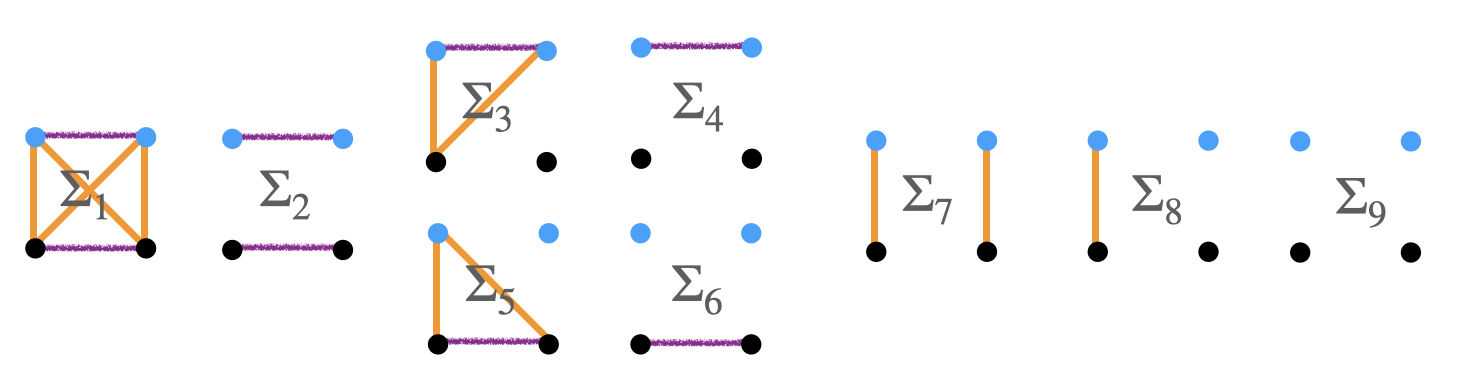
\includegraphics[width=0.3\textwidth]{jacquard.png}  
\end{center}
%\vspace{.1in}
Kinship can be computed from the loading probabilities, $\Delta_j$ for $j$-th latent IBD state $\Sigma_j$, as follows%~\footnote{Jacquard, A. (1972). Biometrics 28(4), 1101–1114.} 
\begin{equation}\label{e1}
\begin{aligned}
\phi &= \Delta_1 + \frac{1}{2}(\Delta_3+\Delta_5+\Delta_7) + \frac{1}{4} \Delta_8.  \\
\end{aligned}
\end{equation}
Inbreeding coefficients can also be computed: 
\begin{equation}\label{e2}
\begin{aligned}
F_1 &= \Delta_1 + \Delta_2 + \Delta_3 + \Delta_4, \\                                                                                                     
F_2 &= \Delta_1 + \Delta_2 + \Delta_5 + \Delta_6. \\
\end{aligned}
\end{equation}

\vspace{-0.2in}
\subsection{Latent states emit joint genotypes}
Each latent IBD states emit joint genotypes at a probability distribution that is a function of allele frequency $p.$%~\footnote{Thompson, E. A. (2013).  Genetics 194(2), 301–326.}
\begin{center} 
\begin{tabular}{lllllllll|ll}
 $\Sigma_1$ &  $\Sigma_2$ &  $\Sigma_3$ &  $\Sigma_4$ &  $\Sigma_5$ &  $\Sigma_6$ &  $\Sigma_7$ &  $\Sigma_8$ &  $\Sigma_9$ &G1 & G2 \\
\hline 
 $p$ & $p^2$ & $p^2$ & $p^3$ & $p^2$ & $p^3$ & $p^2$ & $p^3$ & $p^4$ & AA &AA \\       
 $0$ & $0$ & $pq$ & $2p^2q$ & $0$ & $0$ & $0$ & $p^2q$ &$2p^3q$ &AA &AB  \\
 $0$ & $pq$ & $0$ & $pq^2$ & $0$ & $p^2q$ & $0$ & $0$ &$p^2q^2$ &AA &BB \\
 $0$ & $0$ & $0$ & $0$ & $pq$ & $2p^2q$ & $0$ & $p^2q$ &$2p^3q$ & AB &AA   \\
$0$ & $0$ & $0$ & $0$ & $0$ & $0$ & $2pq$ & $pq$ &$4p^2q^2$ & AB &AB   \\
 $0$ & $0$ & $0$ & $0$ & $pq$ & $2pq^2$ & $0$ & $pq^2$ &$2pq^3$ & AB &BB \\
$0$ & $pq$ & $0$ & $p^2q$ & $0$ & $pq^2$ & $0$ & $0$ &$p^2q^2$ & BB &AA   \\
 $0$ & $0$ & $pq$ & $2pq^2$ & $0$ & $0$ & $0$ & $pq^2$ &$2pq^3$ &BB &AB   \\
 $q$ & $q^2$ & $q^2$ & $q^3$ & $q^2$ & $q^3$ & $q^2$ & $q^3$ & $q^4$ &BB &BB \\       
  \end{tabular} 
  \end{center}
  where $q = 1-p.$ Our aim is to infer $\Delta_j$, the loading probabilities of $\Sigma_j$. 

\vspace{-0.2in}
\subsection{Fit the model}
We consider SNPs with allele frequency $p$ so that they share the same $\Sigma$ matrix.  Denote $\hat\theta$ estimates of fractions of joint genotypes (AA AA, AA AB, ... etc).   
\begin{subequations} \label{lse}
\begin{align}
{\text{arg} \min_\Delta\;\;}  &||\S_p \Delta - \hat\theta_p ||_2  \label{eq:lse} \\
       \mbox{s.t \;\;} \Delta_j & \ge 0  \mbox{\;\;for all $j$, \;and} \sum \Delta_j  = 1 \label{eq:st}
\end{align}
\end{subequations}
where $\S_p = (\Sigma_1, \dots, \Sigma_9)$, $\Delta=(\Delta_1, \dots, \Delta_9)$ is the vector of loading probabilities. 
%
For the $i$-th SNP with allele frequency $p_i$, we can compute $\S_{p_i}$ and we observe $\hat{\theta}=e_i$, where $e_i$ has a single entry $1$ and the rest $8$ entries $0$.  %We append $\S_{p_i}$'s together to obtain the design matrix $\S$ and append $e_i$'s together to obtain a vector $\hat\theta$. For total $m$ SNPs, $\S$ is an $9m \times 9$ matrix, and $\hat\theta$ is an $9m$ vector, and we seek the least square fit of a constrained system
\begin{equation} \label{lse2}
%\begin{aligned}
{\text{arg} \min_\Delta\;\;}  ||\S \Delta - \hat\theta ||_2  %\\
   %    \mbox{s.t \;\;} \Delta_j & \ge 0  \mbox{\;\;for all $j$, \;and} \sum \Delta_j  = 1. 
%\end{aligned}
\end{equation}
with constraints \eqref{eq:st}. We may also fit \eqref{lse2} without constraint. 
%The above system generalizes \eqref{lse} to SNPs of arbitrary allele frequencies.  In practice, we find binning SNPs and re-estimate allele frequencies in each bin improves performance. 


\subsection{Invariant properties}
It can be verified that there are two linear dependence in $\S_p$. One is  $\Sigma_2 + 2 \Sigma_8 = \Sigma_4 + \Sigma_6 + \Sigma_7$ and the other is $pq (\Sigma_1+\Sigma_2- 2\Sigma_3 - 2\Sigma_5 + 2\Sigma_7)  =  \Sigma_7 - 2 \Sigma_8 +  \Sigma_9$. Therefore, the solution to the system $\S \Delta = \hat\theta$ is not unique. Let $\S^{+}$ be Moore-Penrose inverse of $\S$, then $\Delta = \S^{+} \hat\theta + (I - \S^{+} \S) v$ for any vector $v$.  Denote $C = (I - \S^{+} \S) v$,  it can be verified that  
\begin{equation}\label{C}
\begin{aligned}
C_1 =C_3=C_5=C_9 &= 0 \\
C_2  &=  \frac{1}{8} v_2 -  \frac{1}{8} v_4 -  \frac{1}{8} v_6 -  \frac{1}{8} v_7 +  \frac{1}{4} v_8 \\  
C_4 =  C_6 = C_7 &=  - \frac{1}{8} v_2 +  \frac{1}{8} v_4 +  \frac{1}{8} v_6 +  \frac{1}{8} v_7 -  \frac{1}{4} v_8 \\
%C_6 &= - \frac{1}{8} v_2 +  \frac{1}{8} v_4 +  \frac{1}{8} v_6 +  \frac{1}{8} v_7 -  \frac{1}{4} v_8 \\
% C_7 &=   - \frac{1}{8} v_2 +  \frac{1}{8} v_4 +  \frac{1}{8} v_6 +  \frac{1}{8} v_7 -  \frac{1}{4} v_8 \\
  C_8 &= \frac{1}{4} v_2 - \frac{1}{4}  v_4 - \frac{1}{4}  v_6 - \frac{1}{4}  v_7 + \frac{1}{2}  v_8. \\
\end{aligned}
\end{equation}
1)  $\Delta_1, \Delta_3, \Delta_5$, and $\Delta_9$ are not affected by $v$ and these components have unique solutions. 2) $C_2 + C_4 = 0$, $C_2+C_6 = 0$ and $C_7 + \frac{1}{2}C_8 = 0$, which means,  $\Delta_2+\Delta_4 $, $\Delta_2+\Delta_6$, and  $\Delta_7 + \frac{1}{2}\Delta_8$ are invariant. 3) Consequently $\phi$ in Equation~\eqref{e1} and $F_1$ and $F_2$ in Equation~\eqref{e2} are unique. 


\section{Results}
%\vspace{-0.2in}
Software Kindred is available at \url{www.haplotype.org}. 
\vspace{-0.2in}
\subsection{Non-admixed samples}
\begin{center}
\includegraphics[width=0.26\textwidth]{comp3.pdf}
%\includegraphics[width=0.25\textwidth]{comp-j9j3.pdf}
\end{center}

%\vspace{-0.2in}
\subsection{Admixed samples}
\begin{itemize}
\item If the continental population were taken as the homogenous reference population for IBD for non-admixed samples, then for admixed samples 
\item The reference population for IBD for admixed samples has to be the ancestral population predates continental population divergence. 
\item This ancestral population can be partially mimicked by selecting a set of SNPs  whose allele frequencies are similar across different continental populations. 
\item Among 12 million bi-allelic SNPs with minimum 50 minor allele counts (out of total 2504 diplotypes) in 1000 genomes project, there are $1.2$ million such SNPs.  
\item We also randomly selected common bi-allelic SNPs of $1.2$ million,  and used these to compute kinship for comparison. 
\end{itemize}

\begin{center}
\includegraphics[width=0.25\textwidth]{admix-sanguo3.pdf}
\end{center}


\subsection{1000 genomes populations}
%\begin{center}
%\includegraphics[width=0.20\textwidth]{1000g-pop7.pdf}
%\end{center}

\begin{center}
\includegraphics[width=0.24\textwidth]{pairs2.png}\\
\vspace{-0.05in}
{\small Africans (black), Americans (red), East Asians (green), Europeans (blue), and South Asians (cyan).}
\end{center}

\subsection{CenHap on Chr17: Asian vs African}
\begin{center}
\includegraphics[width=0.25\textwidth]{chr17.png}
\end{center}


\subsection{Genomic control}
\begin{center}
\begin{tabular}{lccccccccc}
{$\lambda$} &  {None} &  {scGRM}& {UKin} & {King}    & {Kindred}  & {Kindred$^\pm$}\\
 \hline
lpa & 1.377 & 0.985 & 0.995 & 0.984 & 1.017 & 1.008 \\
pon1 & 1.350 & 0.978 & 0.984 & 0.975 & 1.001 & 0.990 \\
MPO & 1.287 & 0.997 & 0.996 & 1.002 & 1.007 & 1.001 \\
resistin & 1.278 & 0.997 & 0.998 & 1.001 & 1.011 & 1.002 \\
srage & 1.262 & 0.997 & 1.000 & 1.004 & 0.999 & 1.004 \\
cd56 & 1.260 & 0.988 & 0.993 & 0.993 & 1.003 & 0.999 \\
cntn1 & 1.207 & 0.994 & 0.998 & 0.998 & 1.002 & 1.003 \\
CD5L & 1.190 & 1.001 & 1.003 & 1.009 & 1.003 & 1.006 \\
\hline
Mean & 0.276 & 0.008 & 0.005 & 0.008 & 0.005 & 0.004 \\
SSD & 0.064 & 0.007 & 0.005 & 0.008 & 0.006 & 0.003 \\
  \end{tabular}
  \end{center}


\subsection{Heritability of height}

{%\fontsize{26pt}{30}\selectfont
\begin{center}
\begin{tabular}{lccccccc}
  &  {scGRM}& {UKin} & {King}    & {Kindred} & Kindred$^\pm$ \\ 
   \hline
{GCTA}   &0.45  & 0.44 &0.38  &0.47  & 0.41\\
{Gemma} &0.45 & 0.43  & 0.39 &0.47 & 0.41 \\
\hline
90\% & 0.46 &0.45  &0.41  &0.49  & 0.41 \\
70\% & 0.45 &0.47  &0.41  &0.50  & 0.41 \\
50\% & 0.48 &0.49  &0.40  &0.53  & 0.44  \\
%\hline
\end{tabular}
\end{center}
 %Top two rows entries are PVE $\pm$ se estimated from a single dataset of $3925$ samples; Bottom three rows the entries are mean $\pm$ se of 100 independent trials, in each trial PVE was estimated using our Bayesian MAP estimates.
%  In the three resampling studies, 90\%, 70\% and 50\% of the $3925$ samples were sampled without replacement in each trial. 
%We tried to do down-sampling study, but GCTA produced nonsensical results. 

}


\section{Summary}
\begin{itemize}
\item Kindred non-negative estimates for kinship and inbreeding coefficients. 
\item Kindred allows one to specify reference populations. 
\item Kindred works for admixed samples. 
\item Kindred is effective to control for relatedness in GWAS. 
\item Slightly larger but statistically significant estimates of heritability. 
\item Can be extended to infer gene kinship via hidden Markov models. 
\item Software is available at \url{www.haplotype.org}. 
\end{itemize}





\vspace{-.3in}
\begin{thebibliography}{natbib}
%\begin{multicols}{2}
{\small
\bibitem[Jacquard]{}
 Jacquard, A (1972).
%\newblock Genetic information given by a relative.
\newblock {\em Biometrics\/}~{\em 28\/}(4), 1101--1114.

\bibitem[Thompson]{}
Thompson, E.~A. (2013, 06).
%\newblock {Identity by Descent: Variation in Meiosis, Across Genomes, and in Populations}.
\newblock {\em Genetics\/}~{\em 194\/}(2), 301--326.

\bibitem[Wang]{}
Wang, J. (2016, February).
%\newblock Pedigrees or markers: Which are better in estimating relatedness and inbreeding coefficient?
\newblock {\em Theor. Popul. Biol.\/}~{\em 107}, 4--13.

\bibitem[GCTA]{}
Yang, J., S.~H. Lee, M.~E. Goddard, and P.~M. Visscher (2011, 2022/12/25).
%\newblock Gcta: A tool for genome-wide complex trait analysis.
\newblock {\em The American Journal of Human Genetics\/}~{\em 88\/}(1), 76--82.

\bibitem[King]{}
Manichaikul, A., J.~C. Mychaleckyj, S.~S. Rich, K.~Daly, M.~Sale, and W.-M.
  Chen (2010, 10).
%\newblock {Robust relationship inference in genome-wide association studies}.
\newblock {\em Bioinformatics\/}~{\em 26\/}(22), 2867--2873.

\bibitem[UKin]{}
Jiang, W., X.~Zhang, S.~Li, S.~Song, and H.~Zhao (2022).
%\newblock An unbiased kinship estimation method for genetic data analysis.
\newblock {\em BMC Bioinformatics\/}~{\em 23\/}(1), 525.

}
\end{thebibliography}
%\vspace{.2in}


\end{multicols}
\end{document}
